\documentclass[conference,compsoc,a4paper]{IEEEtran}

\usepackage[utf8]{inputenc}
\usepackage[american]{babel}
\usepackage[babel]{csquotes}

\usepackage[final]{pdfpages}
\usepackage[cmex10]{amsmath}
\usepackage{amssymb}
\usepackage{acronym}

\usepackage{xspace}
\usepackage{balance}

\usepackage[
  pdflang=en,
  colorlinks=true,
  unicode=true,
  pdfstartview=,
  allcolors=black
]{hyperref}
\hypersetup{
  pdftitle={Automated Refactoring},
  pdfauthor={Lisa Maria Kritzinger, Peter Feichtinger}
}

\newcommand{\code}[1]{{\small\ttfamily #1}}

\newcommand{\lk}[1]{\textcolor{orange}{[LK] #1}}
\newcommand{\pf}[1]{\textcolor{green}{[PF] #1}}

\newcommand{\JDEvAn}{\mbox{JDEvAn}\xspace}


\begin{document}

\title{Automated Refactoring}
\author{
  \IEEEauthorblockN{Lisa Maria Kritzinger}
  \IEEEauthorblockA{Johannes Kepler University Linz\\
    1255353\\
    Email: \href{mailto:kritzinger@gmx.net}{kritzinger@gmx.net}}
  \and
  \IEEEauthorblockN{Peter Feichtinger}
  \IEEEauthorblockA{Johannes Kepler University Linz\\
    1056451\\
    Email: \href{mailto:shippo@gmx.at}{shippo@gmx.at}}
}

% make the title area
\maketitle


\begin{abstract}
Refactoring, the restructuring of a software system without changing its semantics, is essential in software evolution. 
Manual refactoring can be time-consuming and error-prone, so tool support is desirable when making large changes. In 
this article, we will explore a number of publications on automating different refactoring tasks, from just making code 
more compact to introducing objects into a C codebase.

Additionally, we will provide comparisons which will show the advantages and disadvantages of different approaches, 
regarding the performance of the software after refactoring, the applicability of a certain approach, or the simplicity 
of the application of an approach.


\end{abstract}

\begin{IEEEkeywords}
Software restructuring, automatic refactoring, tool support, software evolution.
\end{IEEEkeywords}

% For peer review papers, you can put extra information on the cover
% page as needed:
% \ifCLASSOPTIONpeerreview
% \begin{center} \bfseries EDICS Category: 3-BBND \end{center}
% \fi
%
% For peerreview papers, this IEEEtran command inserts a page break and
% creates the second title. It will be ignored for other modes.
\IEEEpeerreviewmaketitle


\section{Introduction}

Refactoring is the process of restructuring a software system without changing its semantics. It is used to increase 
readability and maintainability of software, reduce its complexity, or change the architecture of a system. Refactoring 
is essential in software evolution, because as a system is adapted to new requirements it inevitably becomes more 
complex and drifts away from its original design. This makes maintenance more difficult and reduces the software 
quality. Refactoring can then help to bring the system back to its original design and into a more maintainable state, 
improving code quality in the process.

However, manual refactoring without any tool support can be error-prone and time-consuming. There are various tools 
available for supporting elementary refactorings like renaming a variable or introducing an additional parameter to a 
function, often built into the used \emph{Integrated Development Environment} (IDE) itself. But even with tool support, 
manual refactoring can still be too complicated or just tedious, and tool support for automating refactoring tasks is 
desirable in a number of cases.

In this article we're going to highlight some recent and not-so-recent contributions in the field of automatic 
refactoring, ranging from simple tasks like making code more compact \cite{sparta}, to more complicated tasks like 
introducing object-orientation into a C codebase \cite{cpp}.
%We will also investigate the benefit from refactoring a software through replacing conditionals by using polymorphism 
%\cite{polymorphism}, as well as the approach of using design differencing for automated refactoring \cite{design-diff}.


\section{Automated Refactoring Approaches}

This section will give an overview of each paper by summarizing the main points.

\subsection{Restructuring Legacy C Code into C++}

This is an older paper from 1999 by Richard Fanta and Václav Rajlich of \emph{Wayne State University} in Detroit, MI, 
USA~\cite{cpp}. They did a case study on the Mosaic browser, an early web browser implemented in C. Their approach uses 
a number of discrete refactorings. By combining those, a C \code{struct} or a number of related variables can be 
transformed into a C++ class, with related functions becoming member functions of that class.

The following two sections will briefly explain the implemented refactorings and their use in the whole restructuring 
process, respectively.

\subsubsection{Refactoring Tools}

This section briefly summarizes the implemented tools used in the restructuring process. Each tool has specific 
restrictions placed on when it can be applied, which simplifies the tool and makes sure the code is in a consistent 
state after its application.

The \textbf{variable insertion} tool inserts a selected variable into a class as a static or non-static member. The 
programmer needs to specify the variable which should be inserted, as well as the class---for a static variable---or 
the instance---for a non-static variable---it should be inserted into.

Another tool \textbf{makes access to a non-local variable explicit} by introducing an explicit parameter for the 
accessed variable, redirecting all accesses inside the function to that parameter, and finally adding an actual 
parameter for the variable at every call of the function. The same is also possible in reverse to \textbf{make access 
implicit}.

To \textbf{add a parameter} to a function, another tool is used that adds the parameter to the formal parameter list. 
After selecting the instance to be passed as the new parameter for each call, the tool inserts that instance as a 
parameter to the call.

Finally there is a tool for \textbf{changing the access specifier of a class member}, which just checks that a certain 
change doesn't make the code inconsistent.

\subsubsection{Restructuring Scenario}

The refactoring tools described in the previous section are used at various steps in the whole process. The complete 
restructuring process thus involves both actions by a human as well as use of the tools, and is divided into three 
phases.

\begin{enumerate}
  \item Data-only classes are created from a number of variables, if necessary. In case there is already a C 
  \code{struct}, this step can be skipped.
  
  \item After creating the desired classes, possible clones are removed. Clones may result from the same domain concept 
  being implemented at various places in the code.
  
  \item Lastly, the user specifies functions which should be added to a class as a member function. These may be 
  functions that have the target class as a parameter, access it through a global variable, or have individual members 
  of the target class as parameters.
\end{enumerate}

\subsubsection{Results}

They selected a subsystem of 3000 lines from the Mosaic codebase for their tests. Of these 3000 lines they were able to 
encapsulate about 60\% of the code into 12 classes. As an example where clone removal was necessary the give the URL 
class, which was extracted separately at five different locations.

\subsection{Conditionals vs. Polymorphism}

The argument that the cost of refactoring cannot be afforded is often made by programmers, because refactoring usually 
has a negative impact on the performance.

This trade-off has been investigated by Serge Demeyer in 2002 \cite{polymorphism} by comparing the performance of a 
program which contains large conditionals against one where the conditionals were replaced by polymorphic method calls. 
This comparison showed that C++ programs refactored this way perform faster than their non-refactored counterparts.

this approach to refactor a system is mostly suitable for software which contains a large number of conditional logic 
and where performance matters. It is not always possible, or desirable, to replace conditional logic by polymorphism. 
But when the same conditional logic reappears in other pieces of code it becomes a maintenance problem, because one 
risks modifying one condition without adapting the other part as well.

If a client is testing the type of a certain provider object, it can be refactored by moving code from the client to 
the provider. The special case that a client tests whether a provider is \code{null} or empty can be refactored by 
introducing a special \emph{null object} \cite{nullobject}.

The case that an object is testing an attribute serving as some kind of type-tag can be refactored by creating a new 
subclass for each leg of the conditional and moving the code as a polymorphic method into the subclass. If an object is 
changing its state dynamically it can be refactored by introducing a state object \cite[pp.~305--313]{designpatterns}.

Another case are clients which test the type of a series of objects before performing a certain action. This can be 
refactored by a central registration mechanism, which acts as a mediator between objects providing services and clients 
requesting services.

Although this method is easy to use, there is no tool support to automate the process. Therefore it is difficult to 
motivate programmers to make use of this method.

\subsection{Design Differencing}

\begin{figure}[t]
  \centering
    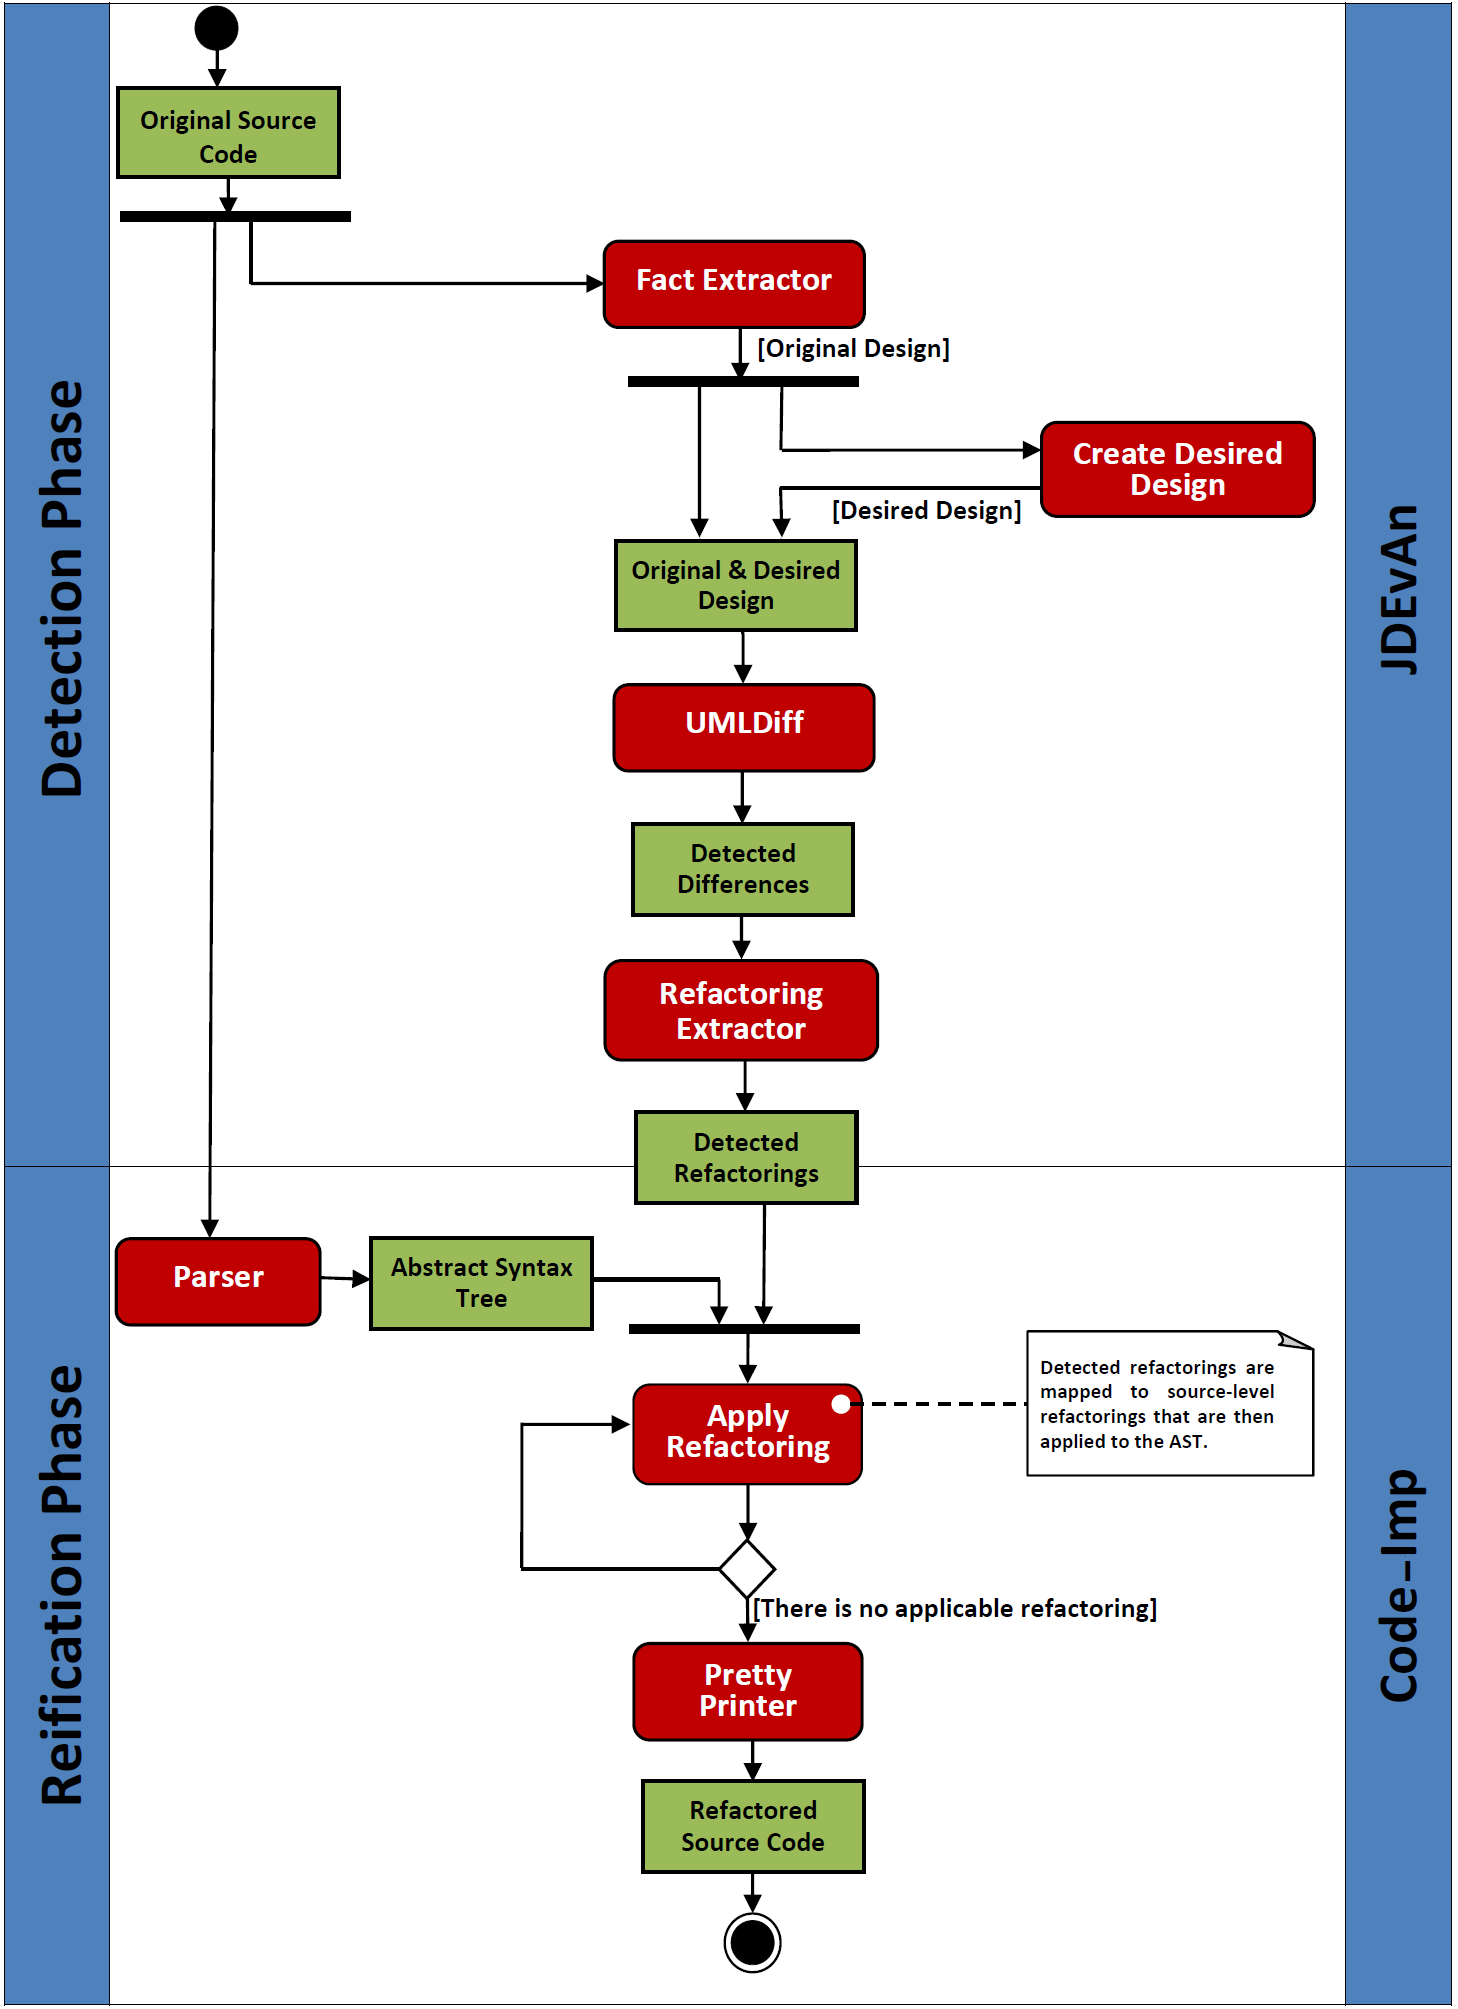
\includegraphics[width=\linewidth]{figures/designdiff.png}
  \caption{Automated refactoring process using Design Differencing \cite{design-diff}}
  \label{fig:designdiff}
\end{figure}

An automated refactoring approach is described in \cite{design-diff}. This novel refactoring approach refactors a 
program based both on its desired design and on its source code.
The process of this method is illustrated in \autoref{fig:designdiff}. The programmer creates a desired design for the 
software. This design shall be based on the current software design and additionally on the understanding of how the 
software may be required to evolve. The software is then refactored using that design. The resulting software code has 
the same behavior as before the refactoring.

This method is supported by some tools, two of them are \JDEvAn (Java Design Evolution and Analysis) \cite{JDEvAn} and 
Code-Imp (Combinatorial Optimization for Design Improvement) \cite{DBLP:journals/jss/OKeeffeC08, 
DBLP:conf/icse/MoghadamC11}.

\subsubsection{JDEvAn}

\JDEvAn is developed at the University of Alberta. It is an Eclipse plugin which analyzes a software system's 
design-evolution history and provides information about the system's history. The plugin contains a Java fact 
extractor, a query-based change-pattern detection module, and a design differencing algorithm. The Java fact extractor 
extracts a UML logical design model from Java source code. The design differencing algorithm uses lexical and 
structural similarity to automatically recover differences between one version of a system and the next \cite{Xing2007}.
\JDEvAn provides a refactoring-detection module which categorizes detected differences as refactoring instances 
\cite{DBLP:conf/wcre/XingS06}.

The process initially extracts two UML models from the source code corresponding to two versions of a Java system. 
Afterwards the two models are compared and the differences between them are detected. Finally the detected differences 
are categorized as design-level refactoring instances. For example, a method which is moved from a class to a subclass 
in the desired design is detected as a number of \emph{move method} differences.

\subsubsection{Code-Imp}

Code-Imp is developed by \cite{DBLP:journals/jss/OKeeffeC08, DBLP:conf/icse/MoghadamC11} as a fully automated 
refactoring framework for automatically improving the design of existing programs. It takes Java source code as input 
and provides a refactored version of the program as output.

The refactoring process of Code-Imp is driven by a search technique. The search technique is steepest-ascent 
hill climbing, where the next refactoring to be applied is the one that produces the best improvement in the so called 
fitness function, a function which measures how good the program is.

The benefit of refactoring software using tools like \JDEvAn and Code-Imp is that it enables automated refactoring 
towards a high-quality desired design, and hence improves maintenance productivity. The efficacy of the approach was 
additionally proven by \cite{design-diff}. Their findings were that the original program could be refactored to the 
desired design with an accuracy of over 90\%, hence demonstrating the viability of automated refactoring using design 
differencing.

\subsection{The Spartanizer}

This is a recent paper by Yossi Gil and Matteo Orrù, which was presented at this year's SANER. It describes their tool 
called \emph{The Spartanizer} \cite{sparta}, which is an Eclipse plugin for automatic refactoring of Java code. The 
tool is still actively being developed on GitHub\footnote{\url{https://github.com/SpartanRefactoring/Main}} and has 
quite a number of contributors.

The supported refactorings are implemented in classes inheriting from the abstract \code{Tipper} class. A tipper 
represents a rewrite rule that can be applied to a specific type of AST node. Multiple tippers can be applied in 
succession to the whole project.

After each modification to a source file, it is parsed and available suggestions are displayed as info markers on the 
source code. From there, it is possible to apply a refactoring to a selected scope (method only, the whole file, etc).

This paper is unique in our list, because it describes a tool that is actively maintained and can be used in 
production, a tool that \enquote{really exists} one could say.


\section{Conclusion}

Text


\section*{Acknowledgments}

Text


\bibliographystyle{IEEEtran}
\bibliography{AutomatedRefactoring}

% TODO Place appropriately
%\balance

% that's all folks
\end{document}
